% % generated by laprint.m
% %
% \begin{psfrags}%
% \psfragscanon%
%
% text strings:
\psfrag{s05}[b][b]{\fontsize{8}{12}\fontseries{m}\mathversion{normal}\fontshape{n}\selectfont \setlength{\tabcolsep}{0pt}\begin{tabular}{c}Magnetic field strength [nT]\end{tabular}}%
\psfrag{s06}[t][t]{\fontsize{8}{12}\fontseries{m}\mathversion{normal}\fontshape{n}\selectfont \setlength{\tabcolsep}{0pt}\begin{tabular}{c}Time [s]\end{tabular}}%
\psfrag{s07}[b][b]{\fontsize{8}{12}\fontseries{m}\mathversion{normal}\fontshape{n}\selectfont \setlength{\tabcolsep}{0pt}\begin{tabular}{c}Magnetic field strength for different sensor pitch angle.\end{tabular}}%
\psfrag{s10}[][]{\fontsize{10}{15}\fontseries{m}\mathversion{normal}\fontshape{n}\selectfont \setlength{\tabcolsep}{0pt}\begin{tabular}{c} \end{tabular}}%
\psfrag{s11}[][]{\fontsize{10}{15}\fontseries{m}\mathversion{normal}\fontshape{n}\selectfont \setlength{\tabcolsep}{0pt}\begin{tabular}{c} \end{tabular}}%
\psfrag{s12}[l][l]{\fontsize{6}{15}\fontseries{m}\mathversion{normal}\fontshape{n}\selectfont $\beta = 90^\circ$}%
\psfrag{s13}[l][l]{\fontsize{6}{15}\fontseries{m}\mathversion{normal}\fontshape{n}\selectfont $\beta = 0^\circ$}%
\psfrag{s14}[l][l]{\fontsize{6}{15}\fontseries{m}\mathversion{normal}\fontshape{n}\selectfont $\beta = 30^\circ$}%
\psfrag{s15}[l][l]{\fontsize{6}{15}\fontseries{m}\mathversion{normal}\fontshape{n}\selectfont $\beta = 60^\circ$}%
\psfrag{s16}[l][l]{\fontsize{6}{15}\fontseries{m}\mathversion{normal}\fontshape{n}\selectfont $\beta = 90^\circ$}%
%
% axes font properties:
\fontsize{6}{15}\fontseries{m}\mathversion{normal}%
\fontshape{n}\selectfont%
%
% xticklabels:
\psfrag{x01}[t][t]{-0.5}%
\psfrag{x02}[t][t]{0}%
\psfrag{x03}[t][t]{0.5}%
%
% yticklabels:
\psfrag{v01}[r][r]{-100}%
\psfrag{v02}[r][r]{-50}%
\psfrag{v03}[r][r]{0}%
\psfrag{v04}[r][r]{50}%
\psfrag{v05}[r][r]{100}%
%
% % Figure:
% \resizebox{6cm}{!}{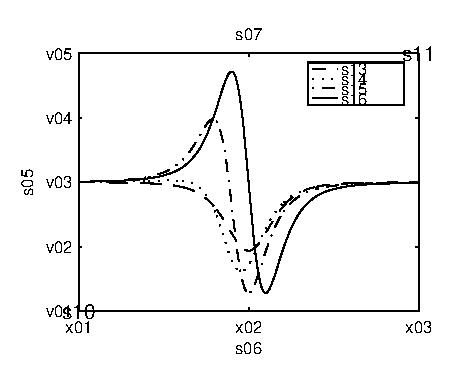
\includegraphics{zrotate.eps}}%
% \end{psfrags}%
% %
% End zrotate.tex
